\documentclass[svgnames,11pt]{beamer}
\input{/home/tof/Documents/Cozy/latex-include/preambule_commun.tex}
\input{/home/tof/Documents/Cozy/latex-include/preambule_beamer.tex}
%\usepackage{pgfpages} \setbeameroption{show notes on second screen=left}
\author[]{Christophe Viroulaud}
\title{Exercices tris\\Correction}
\date{\framebox{\textbf{Algo 05}}}
%\logo{}
\institute{Première - NSI}

\begin{document}
\begin{frame}
\titlepage
\end{frame}
\section{Exercice 1}
\begin{frame}
    \frametitle{Exercice 1}
    \begin{center}    \renewcommand{\arraystretch}{2}

        \begin{tabular}{|c|c|c|}
            \hline
            carré du nombre éléments&$16000^2$&$1000000^2$\\
            \hline
            durée&6,8&\\
            \hline
        \end{tabular}    \renewcommand{\arraystretch}{1}

    \end{center}

    $$\dfrac{6,8×1000000^2}{16000^2}=26560s = 7h23min$$


\end{frame}
\section{Exercice 2}
\begin{frame}[fragile]
    \frametitle{Exercice 2}
\begin{center}
\begin{lstlisting}[language=Python , basicstyle=\ttfamily\small, xleftmargin=0.2em, xrightmargin=0em]
def tri_insertion(tab: list) -> None:
    for i in range(len(tab)):
        # mémoriser
        en_cours = tab[i]
        pos = i
        # décaler
        while pos > 0 and en_cours < tab[pos-1]:
            tab[pos] = tab[pos-1]
            pos = pos-1
        # insérer
        tab[pos] = en_cours
\end{lstlisting}
\begin{lstlisting}[language=Python , basicstyle=\ttfamily\small, xleftmargin=0.2em, xrightmargin=0em]
tab = [randint(0, 100) for _ in range(10)]
tri_insertion(tab)
print(tab)
\end{lstlisting}
\end{center}
    

\end{frame}
\section{Exercice 3}
\begin{frame}
    \frametitle{Exercice 3}

    \begin{center}
        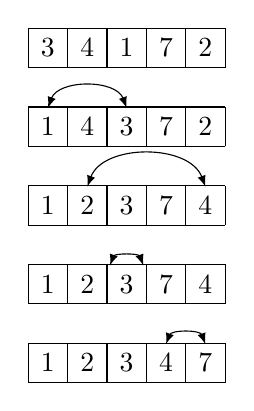
\begin{tikzpicture}[scale=0.5]
            \draw (0,0) grid (5,1);
            \node at(0.5,0.5) {3};
            \node at(1.5,0.5) {4};
            \node at(2.5,0.5) {1};
            \node at(3.5,0.5) {7};
            \node at(4.5,0.5) {2};

            
            \draw (0,-2) grid (5,-1);
            \node (1) at(0.5,-1.5) {1};
            \node at(1.5,-1.5) {4};
            \node (2)at(2.5,-1.5) {3};
            \node at(3.5,-1.5) {7};
            \node at(4.5,-1.5) {2};
            \draw[<->,>=latex] (1.north)to[bend left=70](2.north);

            \draw (0,-4) grid (5,-3);
            \node at(0.5,-3.5) {1};
            \node (3)at(1.5,-3.5) {2};
            \node at(2.5,-3.5) {3};
            \node at(3.5,-3.5) {7};
            \node (4)at(4.5,-3.5) {4};
            \draw[<->,>=latex] (3.north)to[bend left=70](4.north);

            \draw (0,-6) grid (5,-5);
            \node at(0.5,-5.5) {1};
            \node at(1.5,-5.5) {2};
            \node (5)at(2.5,-5.5) {3};
            \node at(3.5,-5.5) {7};
            \node at(4.5,-5.5) {4};
            \draw[<->,>=latex] (5.north west)to[bend left=70](5.north east);
    
            \draw (0,-8) grid (5,-7);
            \node at(0.5,-7.5) {1};
            \node at(1.5,-7.5) {2};
            \node at(2.5,-7.5) {3};
            \node (7)at(3.5,-7.5) {4};
            \node (8)at(4.5,-7.5) {7};
            \draw[<->,>=latex] (7.north)to[bend left=70](8.north);
        \end{tikzpicture}
        \captionof{code}{Tri par sélection}
        \end{center}


\end{frame}
\begin{frame}
    \frametitle{}

    \begin{center}
        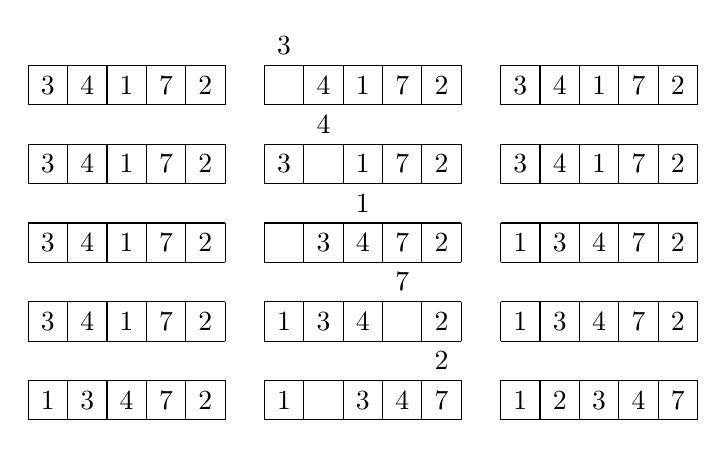
\begin{tikzpicture}[scale=0.5]
            \draw (0,0) grid (5,1);
            \node at(0.5,0.5) {3};
            \node at(1.5,0.5) {4};
            \node at(2.5,0.5) {1};
            \node at(3.5,0.5) {7};
            \node at(4.5,0.5) {2};

            \draw (6,0) grid (11,1);
            \node at(6.5,1.5) {3};
            \node at(7.5,0.5) {4};
            \node at(8.5,0.5) {1};
            \node at(9.5,0.5) {7};
            \node at(10.5,0.5) {2};

            \draw (12,0) grid (17,1);
            \node at(12.5,0.5) {3};
            \node at(13.5,0.5) {4};
            \node at(14.5,0.5) {1};
            \node at(15.5,0.5) {7};
            \node at(16.5,0.5) {2};
            %---
            \draw (0,-2) grid (5,-1);
            \node at(0.5,-1.5) {3};
            \node at(1.5,-1.5) {4};
            \node at(2.5,-1.5) {1};
            \node at(3.5,-1.5) {7};
            \node at(4.5,-1.5) {2};

            \draw (6,-2) grid (11,-1);
            \node at(6.5,-1.5) {3};
            \node at(7.5,-0.5) {4};
            \node at(8.5,-1.5) {1};
            \node at(9.5,-1.5) {7};
            \node at(10.5,-1.5) {2};

            \draw (12,-2) grid (17,-1);
            \node at(12.5,-1.5) {3};
            \node at(13.5,-1.5) {4};
            \node at(14.5,-1.5) {1};
            \node at(15.5,-1.5) {7};
            \node at(16.5,-1.5) {2};
            %---
            \draw (0,-4) grid (5,-3);
            \node at(0.5,-3.5) {3};
            \node at(1.5,-3.5) {4};
            \node at(2.5,-3.5) {1};
            \node at(3.5,-3.5) {7};
            \node at(4.5,-3.5) {2};

            \draw (6,-4) grid (11,-3);
            \node at(7.5,-3.5) {3};
            \node at(8.5,-3.5) {4};
            \node at(8.5,-2.5) {1};
            \node at(9.5,-3.5) {7};
            \node at(10.5,-3.5) {2};

            \draw (12,-4) grid (17,-3);
            \node at(13.5,-3.5) {3};
            \node at(14.5,-3.5) {4};
            \node at(12.5,-3.5) {1};
            \node at(15.5,-3.5) {7};
            \node at(16.5,-3.5) {2};
            %---
            \draw (0,-6) grid (5,-5);
            \node at(0.5,-5.5) {3};
            \node at(1.5,-5.5) {4};
            \node at(2.5,-5.5) {1};
            \node at(3.5,-5.5) {7};
            \node at(4.5,-5.5) {2};

            \draw (6,-6) grid (11,-5);
            \node at(7.5,-5.5) {3};
            \node at(8.5,-5.5) {4};
            \node at(6.5,-5.5) {1};
            \node at(9.5,-4.5) {7};
            \node at(10.5,-5.5) {2};

            \draw (12,-6) grid (17,-5);
            \node at(13.5,-5.5) {3};
            \node at(14.5,-5.5) {4};
            \node at(12.5,-5.5) {1};
            \node at(15.5,-5.5) {7};
            \node at(16.5,-5.5) {2};
            %---
            \draw (0,-8) grid (5,-7);
            \node at(0.5,-7.5) {1};
            \node at(1.5,-7.5) {3};
            \node at(2.5,-7.5) {4};
            \node at(3.5,-7.5) {7};
            \node at(4.5,-7.5) {2};

            \draw (6,-8) grid (11,-7);
            \node at(6.5,-7.5) {1};
            \node at(8.5,-7.5) {3};
            \node at(9.5,-7.5) {4};
            \node at(10.5,-7.5) {7};
            \node at(10.5,-6.5) {2};

            \draw (12,-8) grid (17,-7);
            \node at(12.5,-7.5) {1};
            \node at(13.5,-7.5) {2};
            \node at(14.5,-7.5) {3};
            \node at(15.5,-7.5) {4};
            \node at(16.5,-7.5) {7};
            %---
        \end{tikzpicture}
        \captionof{code}{Tri par insertion}
        \end{center}

\end{frame}
\section{Exercice 4}
\begin{frame}[fragile]
    \frametitle{Exercice 4}

\begin{center}
\begin{lstlisting}[language=Python , basicstyle=\ttfamily\small, xleftmargin=2em, xrightmargin=2em]
def comparer(tab1: list, tab2: list) -> bool:
    for i in range(len(tab1)):
        if not tab1[i] == tab2[i]:
            # stoppe à la première différence
            return False
    # tous les éléments ont été comparés
    return True
\end{lstlisting}
\begin{lstlisting}[language=Python , basicstyle=\ttfamily\small, xleftmargin=2em, xrightmargin=2em]
t1 = [3, 5, 9, 0, 1, 8, 2]
t2 = [9, 5, 3, 2, 8, 1, 0]
tri_insertion(t1)
tri_insertion(t2)
print(comparer(t1, t2))
\end{lstlisting}
\end{center} 

\end{frame}
\section{Exercice 5}
\begin{frame}[fragile]
    \frametitle{Exercice 5}
\begin{center}
\begin{lstlisting}[language=Python , basicstyle=\ttfamily\small, xleftmargin=0.2em, xrightmargin=-2em]
def tri_insertion(tab: list) -> list:
    tab_trie = []
    for i in range(len(tab)):
        # mémoriser
        en_cours = tab[i]
        tab_trie.append(en_cours)
        pos = len(tab_trie)-1
        # décaler
        while pos > 0 and en_cours < tab_trie[pos-1]:
            tab_trie[pos] = tab_trie[pos-1]
            pos = pos-1
        # insérer
        tab_trie[pos] = en_cours
    return tab_trie
\end{lstlisting}
\end{center}
    

\end{frame}
\begin{frame}[fragile]
    \frametitle{}

\begin{center}
\begin{lstlisting}[language=Python , basicstyle=\ttfamily\small, xleftmargin=2em, xrightmargin=2em]
t = [randint(0, 100) for _ in range(10)]
print(tri_insertion(t))
# le tableau initial n'est pas modifié
print(t)
\end{lstlisting}
\end{center}

\end{frame}
\section{Exercice 6}
\begin{frame}[fragile]
    \frametitle{Exercice 6}

\begin{center}
\begin{lstlisting}[language=Python , basicstyle=\ttfamily\small, xleftmargin=0.2em, xrightmargin=0em]
def echanger(tab: list, i: int, j: int) -> None:
    temp = tab[i]
    tab[i] = tab[j]
    tab[j] = temp

def inserer(tab: list, j: int) -> None:
    # Le changement se fait dans la comparaison
    while j-1 >= 0 and tab[j-1][0] > tab[j][0]:
        echanger(tab, j-1, j)
        j = j-1

def tri_insertion(tab: list) -> None:
    for i in range(len(tab)):
        inserer(tab, i)
\end{lstlisting}
\end{center}    
\begin{aretenir}[]
Le tri par insertion est stable. Ce n'est pas le cas du tri par sélection.
\end{aretenir}
\end{frame}
\section{Exercice 7}
\begin{frame}[fragile]

\begin{center}
\begin{lstlisting}[language=Python , basicstyle=\ttfamily\small, xleftmargin=0.2em, xrightmargin=-3em]
def max_occurrences(tab: list) -> tuple:
    tri_insertion(tab)
    # départ 1° série
    en_cours = tab[0]
    serie_en_cours = 1
    elt_max = tab[0]
    serie_max = 1
    for i in range(1, len(tab)):
        # cas même élément que le précédent
        if en_cours == tab[i]:
            serie_en_cours += 1
        else:
            # vérifie alors la taille de la dernière série
            if serie_en_cours > serie_max:
                serie_max = serie_en_cours
                elt_max = en_cours
            # départ nouvelle série
            en_cours = tab[i]
            serie_en_cours = 1
    return (elt_max, serie_max)
\end{lstlisting}
\end{center} 

\end{frame}
\begin{frame}[fragile]
    \frametitle{}

\begin{center}
\begin{lstlisting}[language=Python , basicstyle=\ttfamily\small, xleftmargin=0.2em, xrightmargin=-2em]
t = [randint(0, 10) for _ in range(100)]
maxi = max_occurrences(t)
print(f"Le nombre {maxi[0]} est apparu {maxi[1]} fois.")
\end{lstlisting}
\end{center}

\end{frame}
\section{Exercice 8}
\begin{frame}[fragile]
    \frametitle{Exercice 8}

\begin{center}
\begin{lstlisting}[language=Python , basicstyle=\ttfamily\small, xleftmargin=0.2em, xrightmargin=0em]
def echanger(tab: list, i: int, j: int) -> None:
    """
    échange deux éléments de tab
    """
    temp = tab[i]
    tab[i] = tab[j]
    tab[j] = temp
\end{lstlisting}
\end{center}

\end{frame}
\begin{frame}[fragile]
    \frametitle{}

\begin{center}
\begin{lstlisting}[language=Python , basicstyle=\ttfamily\small, xleftmargin=0.2em, xrightmargin=0em]
def tri_bulles(tab: list) -> None:
    for i in range(len(tab)):
        # on s'arrête avant la partie déjà triée
        for j in range(1, len(tab)-i):
            # remonte l'élément le plus grand
            if tab[j-1] > tab[j]:
                echanger(tab, j-1, j)
\end{lstlisting}
\end{center} 

\end{frame}
\end{document}